\chapter{Kosmické záření v blízkém okolí Země}
Ionizující záření ve vesmíru je tvořeno širokou škálou primárních částic s velkým rozsahem energií. Tok těchto částic je zpravidla malý. Při průchodu látkou (kosmická loď, povrch ISS a její obsah) vznikají nabité a neutrální sekundární částice, jejichž přítomnost hraje roli při výběru vhodného typu stínění kosmické lodi, vesmírných stanic atp.   

Kosmickým zářením v blízkém okolí Země rozumíme ionizující záření v tomto okolí. Na obr. \ref{fig:zdroje} vidíme tři hlavní zdroje tohoto ionizujícího záření: (1) galaktické kosmické záření (GCR-galactic cosmic rays), což je proud nabitých částic, které vznikly mimo sluneční soustavu; (2) energetické elektrony a protony zachycené v geomagnetickém poli tvořící radiační pásy Země, též nazývané Van Allenovy pásy (ERB, Earth's radiation belts); (3) sluneční události s emisí částic (SPE, solar particle events), vysoké toky nabitých částic emitovaných během vzácných, ale intenzivních slunečních erupcích (solar flares) nebo výronech koronální hmoty (CME, coronal mass ejections) \cite{benton}. Někdy se udávají jako čtvrtá složka albedo neutrony a protony, což jsou sekundární částice
vzniklé při interakcích mezi GCR a zemskou atmosférou s trajektorií mířící zpět do vesmíru. Avšak příspěvek albedo částic je malý, a proto se většinou neuvažuje.

\begin{figure}[ht]
  \centering
  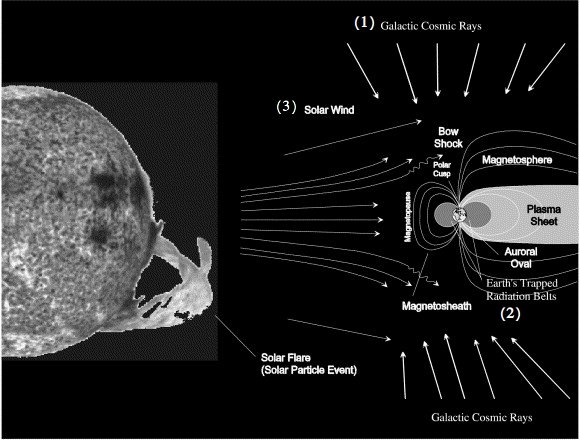
\includegraphics[width=0.7\textwidth]{zdroje.jpg}
  \caption{Tři hlavní zdroje kosmického záření v blízkosti Země: (1) galaktické kosmické záření, (2) zachycené částice v radiačních pásech Země a (3) sluneční události s emisí částic. Z obrázku je dále zřejmé, že všechny tři zdroje jsou ovlivňovány zemským magnetickým polem. \cite{benton}}
  \label{fig:zdroje}
\end{figure}

V dalším textu nejprve stručně rozebereme jednotlivé zdroje kosmického záření v blízkém okolí Země, poté se podíváme, jaké faktory ho ovlivňují.
\section{Zdroje kosmického záření v blízkém okolí Země}
\subsection{Galaktické kosmické záření}
Galaktické kosmické záření se skládá z 98 \% z protonů a těžších iontů (baryonová složka), z 2 \% z elektronů a pozitronů (leptonová složka). V baryonové složce převládají protony (87\%) a alfa částice (12\%), zbytek tvoří ionty s protonovým číslem od 3 (Li) do 92 (U) \cite{benton}. Důležitou roli ve vesmírné dozimetrii hrají částice s velkým atomovým číslem a velkou energií, jelikož jsou celkem hojné a mají velikou pronikavost.

Tok kosmického záření, které vstupuje do sluneční soustavy a zároveň nemá energii větší než cca 1 GeV, je zeslabováno slunečním větrem. Intenzita tohoto zeslabení se odvíjí od jedenáctiletého slunečního cyklu: k největšímu zeslabení dochází při slunečním maximu, naopak při slunečním minimu je zeslabení nejmenší. 

Kosmické záření je dále ovlivňováno zemským magnetickým polem. Nabité částicí tíhnou ke sledování geomagnetických siločar, které jsou paralelní k zemskému povrchu v oblasti kolem rovníku a do Země se vnořují v oblasti u pólů. Proto je většina částic (až na ty nejvíce energetické) odnášeno pryč od rovníku a u polů jsou propouštěny k povrchu (to je příčinou existence např. polární záře). Z toho vyplývá, že vesmírné lodě a stanice získávají největší ozáření od GCR blízko pólů.

\subsection{Zemské radiační pásy}
Zemské radiační pásy jsou vrstvy protonů a elektronů rozprostírajících se kolem Země. Tyto částice jsou zachyceny geomagnetickým polem a pohybují se vícero způsoby (obr. \ref{fig:ERBs}): rotace částic kolem geomagnetickým siločar se nazývá cyklotronový pohyb; vzhledem k nerovnoměrnosti zemského magnetického pole se částice pohybují podél jeho siločar (u pólů mění směr); jako poslední pohyb je udáván drift částic kolem Země (protony driftují na západ a elektrony na východ).

\begin{figure}[H]
  \centering
  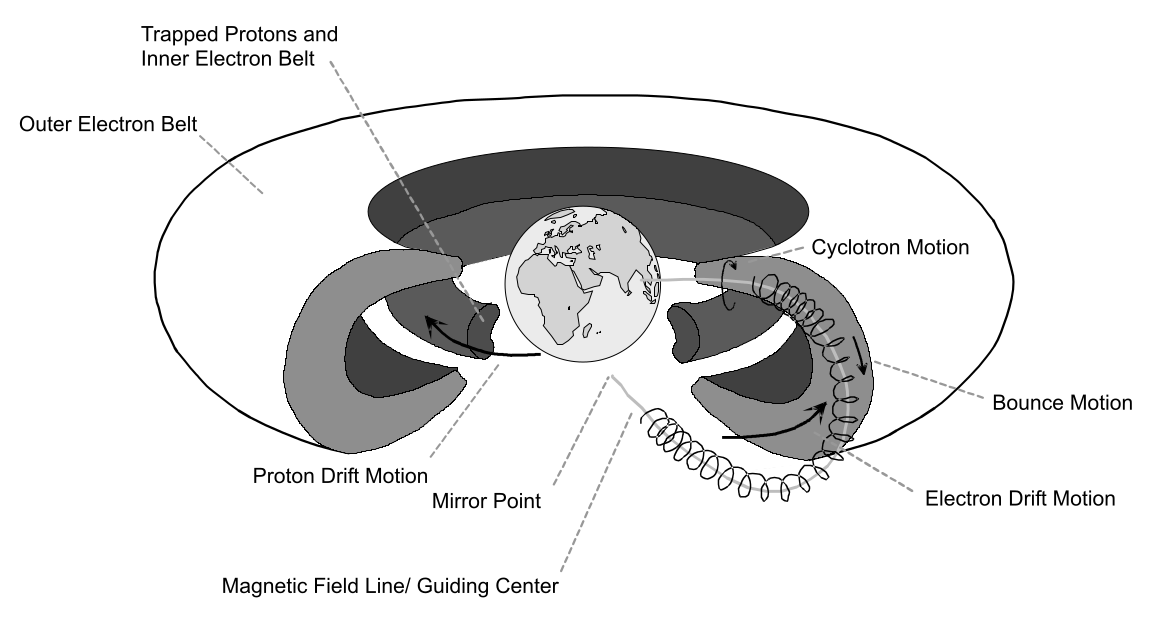
\includegraphics[width=0.8\textwidth]{ERBs.png}
  \caption{Radiační pásy Země, nabité částice se pohybují třemi způsoby: cyklotronový pohyb, posuvný pohyb podél siločar a driftový pohyb kolem Země. \cite{benton}}
  \label{fig:ERBs}
\end{figure}

Zachycené elektrony se nacházejí ve dvou vrstvách a vzhledem k jejich převážně nízké energii nepředstavují veliký zdravotní risk. Zachycené protony se nacházejí v jedné oblasti a jejich intenzita klesá s rostoucí vzdáleností od Země. Jejich energie se pohybuje v řádech od jednotek do stovek MeVů, přičemž maximum nastává při hodnotě z intervalu [150, 250] Mev. Protože se oběžná dráha ISS nachází v menší nadmořské výšce, než ve které je většina zachycených protonů, nepřispívají protony významněji k celkové dávce ISS. Výjimku představuje tzv. jihoatlatická anomálie (SAA, south Atlantic Anomaly), která se rozprostírá nad pobřežím Brazílie; v tomto místě dochází k přiblížení zachycených protonů k zemskému povrchu, což je důsledek netotožnosti geografických a magnetických zemských pólů.
Vrstva zachycených protonů zde protíná oběžnou dráhu ISS (a dalších vesmírných projektů); dávku ISS při průchodu SAA (tedy pro sklon 51,56$^\circ$ a nadmořskou výšku cca 400 km oběžné dráhy ISS)  tvoří zhruba z poloviny zachycené protony a z poloviny GCR (při větší zeměpisné šířce) \cite{benton}. 

\subsection{Sluneční události s emisí částic}
Tento zdroj ionizujícího záření zahrnuje částice emitované ze slunce během slunečních erupcí nebo výronech koronální hmoty (CME), tj. protony, elektrony a těžší nabité částice (do železa). Sluneční události s emisí částic jsou celkem vzácné a vyskytují se hlavně během slunečního maxima. Během jednoho slunečního cyklu se dá očekávat cca 50 událostí, přičemž jedna či dvě mohou být většího charakteru (fluence protonů je větší než 10$^{10}$ cm$^{-2}$).

Na obrázku \ref{fig:SPEs} vidíme rozdíl mezi sluneční erupcí a CME. Sluneční erupce je krátko žijící, obvykle v řádu hodin, a je charakteristická relativně velkými toky elektronů. Celková fluence je malá, mezi 10$^7$ a 10$^8$ cm$^{-2}$ a tyto události jsou omezeny na 30-40$^\circ$ solární délky. Druhý typ SPE, výron koronální hmoty, je déle žijící, přežívá v řádu dnů. Je charakteristická mnohem většími toky protonů, totální fluence může přesáhnout 10$^9$ cm$^{-2}$ a může se šířit pod širokým úhlem solární délky, od 60$^\circ$ až do 180$^\circ$ \cite{benton}.

\begin{figure}[H]
  \centering
  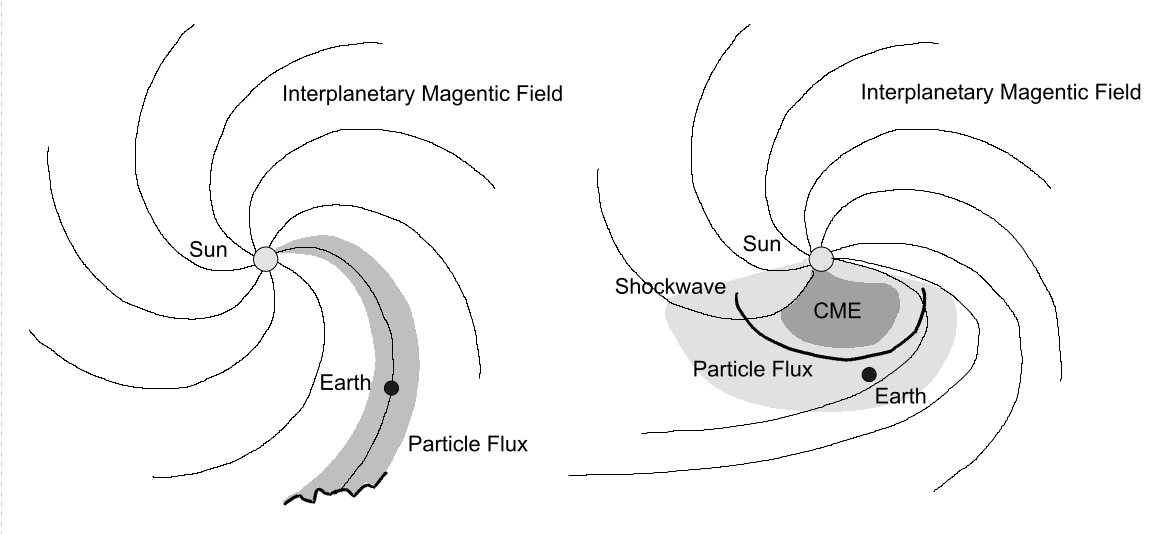
\includegraphics[width=0.75\textwidth]{SPEs.png}
  \caption{Dva typy SPEs: nalevo je sluneční erupce a napravo CME. \cite{benton}}
  \label{fig:SPEs}
\end{figure}

Časový vývoj typické SPE začíná prudkým nárůstem toku, maxima je dosaženo v řádu minut až hodin. Poté dochází k pozvolnému klesání, též v řádu minut až hodin, následované možným druhým maximem, který vzniká, když meziplanetární šoková vlna míjí Zem (v případě CME).

Ovšem k významnějšímu zvýšení dávkového příkonu v blízkém okolí Země od SPE musí být splněno několik podmínek. SPE musí mít velikou celkovou fluenci, dále se musí vyskytnout v takové solární délce, která je propojena se Zemí meziplanetárním magnetickým polem, a nakonec jí nesmí minout. Dále zde musí být správné podmínky geomagnetického pole, aby částice od SPE nebyly odneseny pryč. Záleží také na nadmořské výšce oběžné dráhy sledovaného kosmického tělesa -- pokud totiž leží pod geomagnetickým polem (nebo alespoň nějakou jeho vrstvou), pak je jím chráněno.
\subsection{Sekundární částice}
Většina ztrát energie primárních částic při průchodu látkou je ve formě ionizace, avšak mnoho primárních částic má velkou energii, a proto může část z nich podstoupit jaderné reakce s jádry látky (vesmírná stanice a její obsah), čímž se produkují sekundární částice. Pokud mají sekundární částice dostatečnou energii, pak mohou stejným způsobem produkovat další částice - to se děje zvláště u vysokoenergetických neutronů.

Důležité jsou dva typy jaderných interakcí: fragmentace terčového jádra a fragmentace projektilu. Při první z nich dochází k rozštěpení terčíku; tato interakce nastává při srážce vysokoenergetické primární nabité částice, obvykle GCR nebo zachyceného protonu, a těžkého jádra, obvykle Al jádra stanice nebo C a O lidského těla. Při druhém typu dochází k rozštěpení nalétavájícího projektilu; tato interakce nastává při srážce těžké nabité částice s terčíkem. V obou případech se produkuje jedna či více sekundárních částic, např. protony, neutrony, $\alpha$ částice, těžká jádra; při druhém typu navíc může dojít ke vzniku většího štěpného fragmentu, který pak odnáší většinu kinetické energie~\cite{benton}. 
 
%Tvorba sekundárních částic velmi souvisí se stíněním stanice/satelitu.

%\begin{figure}[H]
  %\centering
  %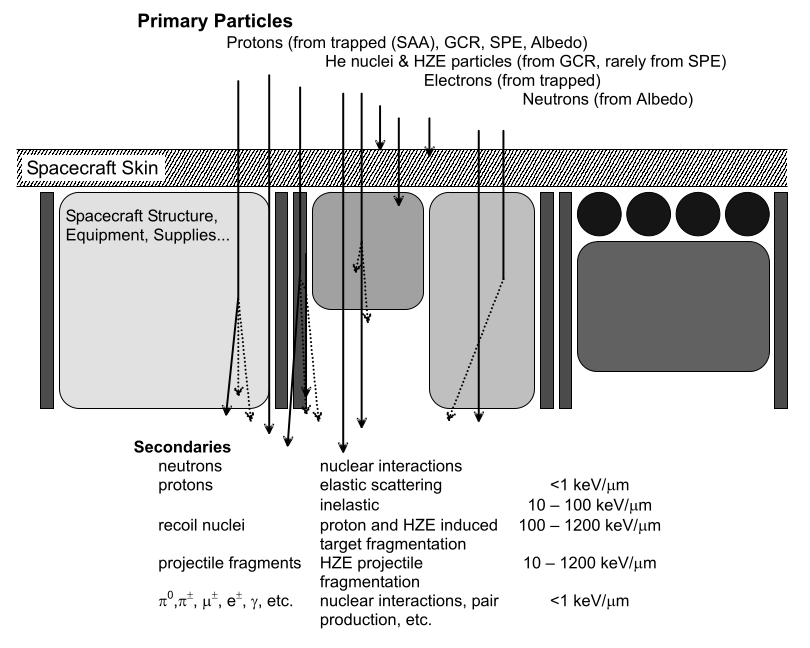
\includegraphics{sekundarniCastice.png}
  %\caption{<+caption text+>}
  %\label{fig:sekundarniCastice}
%\end{figure}

%K první z nich dochází při srážce vysokoenergetické primární nabité částice, obvykle GCR nebo zachyceného protonu, a těžkého jádra, obvykle Al jádra stanice nebo C a O lidského těla. Produkuje se jedna či více sekundárních částic, např. protony, neutrony, $\alpha$ částice, těžká jádra.
%K druhému typu dochází pri srážce HZE s terčíkem, produkují se znovu protony, neutrony atd. a navíc může dojít ke vzniku většího štěpného fragmentu, který pak odnáší většinu kinetické energie. 
%Tvorba sekundárních neutronů je úzce spjatá se stíněním primárního záření
%nevím jestli psát o sekundárních neutronech na tomto místě ..
\section{Faktory ovlivňující kosmické záření v blízkém okolí Země}
\subsection{Fáze slunečního cyklu}\label{sec:kosmickeZareni_solar}
Se zvyšující se solární aktivitou klesají příspěvky od GCR a od protonů zachycených v SAA k celkové obdržené dávce. Je to dáno odklonem ionizujících částic, který je způsoben meziplanetárním magnetickým polem \cite{dosis}.
\subsection{Sklon oběžné dráhy}
Relativní příspěvek GCR a zachycených protonů k celkovému záření, jemuž je vesmírný objekt vystaven v LEO, je ovlivněn inklinací oběžné dráhy stanice/satelitu vzhledem k zemskému rovníku. Pro velké sklony oběžné dráhy (tedy takové, které zanášejí objekt blízko magnetickým polům) převládá složka galaktického kosmického záření, protože GCR částice jsou geomagnetickým polem zanášeny blíže k Zemi a protože průměrný čas zabírající překonání jihoatlatické anomálie je malý ve srovnání s orbitální periodou. Naopak pro malé sklony oběžné dráhy (blízko rovníku) je největším zdrojem záření jihoatlatická anomálie, k čemuž přispívá i geomagnetické pole, jež většinu GCR částic odnáší pryč od rovníku.
\subsection{Nadmořská výška}\label{sec:kosmickeZareni_altitude}
Ozáření vesmírného objektu je silně závislé na nadmořské výšce: s rostoucí nadmořskou výškou roste i dávkový příkon; pokud se objekt nachází nad SAA, pak je růst exponenciální (do určitých výšek). Tato závislost je způsobena hlavně protony zachycenými v ERBs; naopak ozáření pocházející od GCR je na nadmořské výšce v podstatě nezávislé \cite{dosis}.
\subsection{Východní/západní anizotropie zachycených protonů}\label{sec:kosmickeZareni_anizotropie}
Tok protonů vstupujících do vesmírného objektu nad SAA je anizotropní: protony pohybující se na východ následují geomagnetické siločáry ležící nad oběžnou dráhou objektu, zatímco protony pohybující se na západ následují geomagnetické siločáry ležící pod oběžnou dráhou objektu. Poloměr cyklotronového pohybu protonů v SAA %je stejného řádu jako výška atmosféry
je přímo úměrný atmosférickému měřítku výšky (atmospheric density scale height); tato veličina je definovaná jako vzrůst v nadmořské výšce, pro který se atmosférický tlak sníží o faktor~e~\cite{scaleHeight_wiki}. Ona úměrnost je způsobena tím, že protony cestující na západ se pohybují v hustší vrstvě atmosféry a tudíž s větší pravděpodobností interagují s atmosférou, čímž je toto záření utlumeno. Tento jev se projevuje až trojnásobným rozdílem dávkového příkonu mezi západní (do které narážejí protony cestující na východ) a východní (protony cestující na západ) částí objektu \cite{benton}. 
\subsection{Stínění}
Stínění vesmírného objektu představuje jeden z nejdůležitějších faktorů ovlivňující charakter záření uvnitř vesmírného objektu. Zvyšením stínění se dosáhne snížení dávkového příkonu uvnitř objektu, avšak na druhou stranu se zvýší jakostní činitel záření $Q$, tedy potenciální nebezpečnost záření z hlediska zdraví astronautů. Vzrůst $Q$ je dán zpomalením primárních částic ve stínění, které vede ke zvýšení jejich LET (Linear energy tranfer, lineární přenos energie) \cite{toNemecky}.

Tento jev lze pozorovat např. v měřeních prováděných univerzitou v San Franciscu v letech 1996-1997 na palubě ruské kosmické stanice Mir. Obr. \ref{fig:stineni} zobrazuje dvě LET spektra. Obě dvě byla naměřena detektory stop CR-39, přičemž jeden detektor byl silně stíněn (více než 40 g/cm$^2$) a druhý pouze slabě (méně než 20 g/cm$^2$). Pro LET menší než cca 100 keV/$\mu$m obě jsou spektra velmi podobná, nicméně pro větší hodnoty LET leží spektrum prvního detektoru znatelně výš než spektrum druhého detektoru \cite{benton}. To plně odpovídá informacím z prvního odstavce.
\begin{figure}[H]
  \centering
  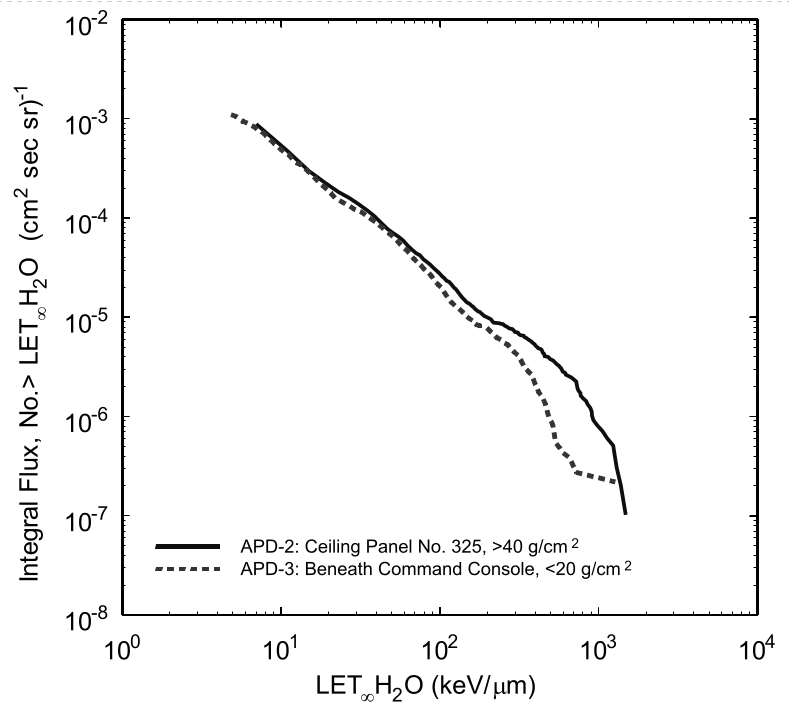
\includegraphics[width=0.6\textwidth]{stineni.png}
  \caption{Integrální LET spektra měřená na dvou různě odstíněných místech v kosmické stanici Mir v roce 1997 \cite{benton}. Plná čára zobrazuje spektrum silně stíněného detektoru, čárkovaná slabě stíněného detektoru.}
  \label{fig:stineni}
\end{figure}

Ve stínění dále mohou vznikat sekundární částice (ty ale mohou vznikat i uvnitř objektu), které v závislosti na tloušťce stínění mohou, ale nemusejí být pohlceny v samotném stínění; v případě nepohlcení představují taktéž určitý zdravotní risk~\cite{benton}. 
%, případně ke vzniku sekundárních částic, které se v závislosti na tloušťce stínění mohou a nemusí pohltit ve stínění.

%Čím větší stínění, tím je spektrum záření uvnitř objektu tvrdší, tj. záření je více energetické; naopak zmenšováním stínění roste dávkový příkon. Příčinou je tvorba sekundárních částic v materiálu stínění.

%Stínění objektu dále velmi souvisí s produkcí sekundárních částic.
%tady je toho málo; kousek tam nechápu
